\section{Network Flow}

\begin{frame}
  \begin{center}
    {\bf Part IV - Network Max Flow}
  \end{center}
\end{frame}

\begin{frame}
  \frametitle{Network Max Flow -- Problem Definition}

  \begin{block}{}
    Consider a {\bf weighted} network of pipes. The weight is the size of each pipe. Water enters the network at $v_s$ and leave at $v_t$. How much water is leaving through $v_t$?
  \end{block}

  \begin{center}
    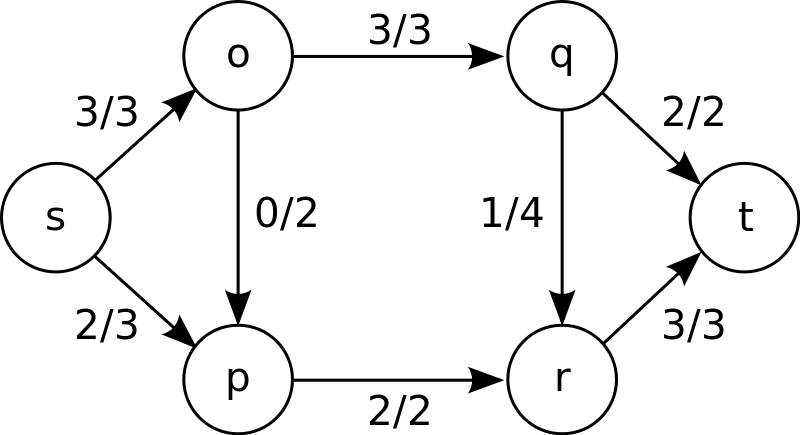
\includegraphics[width=.45\textwidth]{../img/maxflow_wiki}
    \ppagenote{Network Flow Image CC-BY-SA 3.0 by Maksim}
  \end{center}

  \begin{itemize}
    \item 2 units come through $s\to o \to q \to t$,
    \item 2 units come through $s\to p\to r\to t$,
    \item 1 unit comes through $s\to o\to q\to r\to t$.
  \end{itemize}
\end{frame}

\begin{frame}
  \frametitle{Network Max Flow -- Problem Definition}
  \begin{center}
    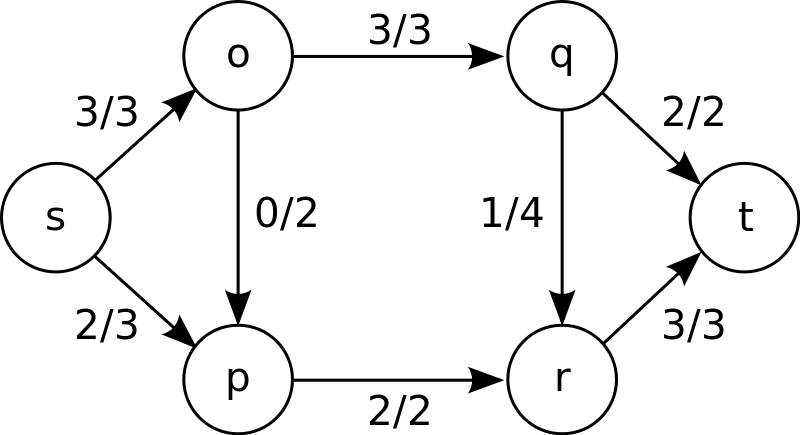
\includegraphics[width=.55\textwidth]{../img/maxflow_wiki}
  \end{center}
  \bigskip

  The goal of the Max Flow problem is to find the maximum total flow that can go between $v_s$ and $v_t$ in a given graph.
\end{frame}


\begin{frame}[fragile]
  \frametitle{Ford Fulkerson Method for Max Flow}

  \begin{block}{}
    The Ford-Fulkerson method\footnote{Same Ford as in Bellman-Ford} finds the maximum flow using a {\bf Residual Flow Graph} to keep track of remaining capacity.
  \end{block}

  \medskip

  \begin{itemize}
  \item {\bf Initialize Residual Graph F}: equal to the original graph G, but directed (add edges as necessary)\medskip
  \item {\bf Main Loop:} If there is a path $p$ between $v_s$ and $v_t$ in F:
  \begin{itemize}
    \item Find smallest weight $w$ in p;
    \item For every edge $E_{u,v} \in p$, {\bf subtract} w from each edge;
    \item For every back-edge $E_{v,u} | E_{u,v}\in p$, {\bf add} w to each edge;
    \item Find another path $v_s \to v_t \in F$
  \end{itemize}
  \end{itemize}
\end{frame}

\begin{frame}[fragile]
  \frametitle{Ford Fulkerson -- Pseudocode}
% {\smaller
  \begin{exampleblock}{}
\begin{verbatim}
int residual[V][V];                   // Initialize Residual Graph
memset(residual, 0, sizeof(residual))
for (int i; i < V; i++)
  for (int j; j < V; j++)
    residual[i][j] = AdjMat[i][j];
mf = 0;                               // Max flow counter
while (P = FindPath(s, t)) {          // Find new path;
   m = P.min_weight;                  // minimum edge in P
   for (edge (v,u) in P) {
      residual[v][u] -= m;
      residual[u][v] += m;
   }
   mf += m;
}
\end{verbatim}
  \end{exampleblock}
  % }
\end{frame}

\begin{frame}{Ford-Fulkerson Simulation}
  \begin{tikzpicture}[transform shape,label/.style={thin, draw=black, align=center,fill=white,font=\smaller},scale=1.1]
    \node[vertex] (0) at (0,0) {s};
    \node[vertex] (1) at (1.5,1.5) {1};
    \node[vertex] (2) at (1.5,-1.5) {2};
    \node[vertex] (3) at (3,1.5) {3};
    \node[vertex] (4) at (3,-1.5) {4};
    \node[vertex] (5) at (4.5,0) {t};
    \draw[edge] (0) to node[label] {3} (1);
    \draw[edge] (0) to node[label] {2} (2);
    \draw[edge] (1) to node[label] {2} (2);
    \draw[edge] (1) to node[label] {3} (3);
    \draw[edge] (2) to node[label] {2} (4);
    \draw[edge] (3) to node[label] {4} (4);
    \draw[edge] (3) to node[label] {2} (5);
    \draw[edge] (4) to node[label] {3} (5);
  \end{tikzpicture}
  \vspace{10cm}
\end{frame}

\begin{frame}{Finding Paths in Ford Fulkerson -- Problems}

The Ford Fulkerson method does not specify an algorithm for finding a path in the residual graph. You could use anything!\bigskip

\begin{exampleblock}{Problem case with bad path finding}
  The worst case of path selection could be $O(|f^*|E)$, where $f^*$ is the true Max Flow value.\medskip

  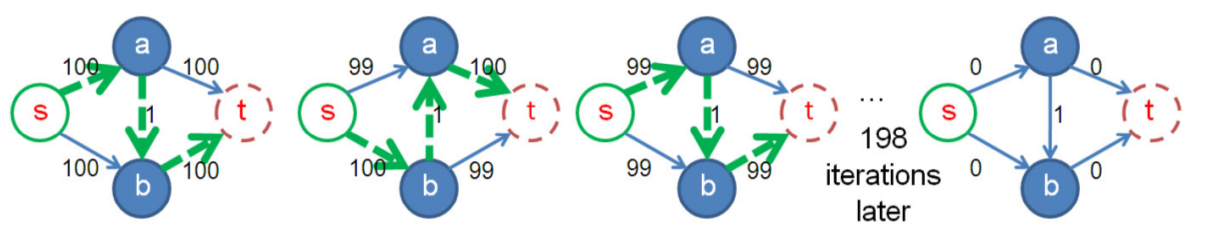
\includegraphics[width=1\textwidth]{../img/ff_worst_halim}
  \ppagenote{Image from "Competitive Programming 3", Steven Halim}
\end{exampleblock}
\end{frame}

\begin{frame}[fragile]
  \frametitle{FF efficient implementation: Edmond Karp's Algorithm}

  \begin{block}{}
    To avoid these "worst cases" of bad path selection, {\bf Edmond Karp}'s algorithm uses BFS on the residual graph to select a new $s\to t$ path.
  \end{block}

{\smaller
\begin{block}{Pseudocode}
\begin{verbatim}
boolean BFS(s, t, p) { } // Finds shortest (by edge #) path from s to t and store in p

mf = 0
while BFS(s,t,p) do {
  for (i in p) {
    minw = min(minw, p[i].w) // find min in p;
  }
  mf += minw;
  for (i in p) {
    res[p[i].u][p[i].v] -= minw;
    res[p[i].v][p[i].u] += minw;
  }
}
\end{verbatim}
\end{block}
}
\end{frame}


\subsection{Maxflow Problem Example}
\begin{frame}
  \frametitle{Example: Software Allocation}
    \begin{block}{Outline}
      In a laboratory there are 26 applications and 10 computers. Each computer can run a subset of these applications. Each computer can run only one program per day.\bigskip

      Every day, laboratory users submit {\bf application requests}. These requests can be repeated. For example, two users can request application A, and one user requests application B.

      You must determine if it is possible to satisfy all applications. If so, you must print the computer allocation.
    \end{block}

    \bigskip
    {\bf QUIZ:} How do you solve this program?
\end{frame}

\begin{frame}{Example: Software Allocation}

    {\bf Allocation Problems} (also called ``matching''
    problems) can usually be solved using Max Flow.
    \bigskip

    The main part of the problem is: {\bf What is the graph that best represents this problem?}

    \begin{itemize}
      \item Create a {\bf source vertex s} connected to all applications.
      \begin{itemize}
        \item The weight of these edges is the number of users requesting that application.
      \end{itemize}\medskip
      \item Create an edge connecting each application to the computers that can run that application.\medskip
      \item Create an edge connecting each computer to a {\bf sink vertex t}.
      \begin{itemize}
        \item The weight of these edges is 1 (number of programs that can run on the computer).
      \end{itemize}
    \end{itemize}\bigskip

    Solve the maxflow problem for this graph. If the flow size is equal to the number of users, then the allocation is satisfied.
\end{frame}

\begin{frame}{Example: Software Allocation}{Input Example One}
A4 01234;\\
Q1 5;\\
P4 56789;\\


   \begin{center}
     \begin{tikzpicture}[transform shape,label/.style={thin, draw=black, align=center,fill=white,font=\smaller},scale=1.1]
       \tikzset{edge/.style = {->,>=latex'}}
       \node[red vertex] (s) at (0,0) {s};
       \node[vertex] (A) at (-2,-1) {A};
       \node[vertex] (Q) at (0,-1) {Q};
       \node[vertex] (P) at (2,-1) {P};
       \node[vertex] (0) at (-4,-3) {0};
       \node[vertex] (1) at (-3,-3) {1};
       \node[vertex] (2) at (-2,-3) {2};
       \node[vertex] (3) at (-1,-3) {3};
       \node[vertex] (4) at (0,-3) {4};
       \node[vertex] (5) at (1,-3) {5};
       \node[vertex] (6) at (2,-3) {6};
       \node[vertex] (7) at (3,-3) {7};
       \node[vertex] (8) at (4,-3) {8};
       \node[vertex] (9) at (5,-3) {9};
       \node[red vertex] (t) at (0,-4) {t};
       \draw[edge] (s) -- node[label] {4} (A);
       \draw[edge] (s) -- node[label] {1} (Q);
       \draw[edge] (s) -- node[label] {4} (P);
       \draw[edge] (A) -- (0);
       \draw[edge] (A) -- (1);
       \draw[edge] (A) -- (2);
       \draw[edge] (A) -- (3);
       \draw[edge] (A) -- (4);
       \draw[edge] (Q) -- (5);
       \draw[edge] (P) -- (5);
       \draw[edge] (P) -- (6);
       \draw[edge] (P) -- (7);
       \draw[edge] (P) -- (8);
       \draw[edge] (P) -- (9);
       \draw[edge] (0) -- (t);
       \draw[edge] (1) -- (t);
       \draw[edge] (2) -- (t);
       \draw[edge] (3) -- (t);
       \draw[edge] (4) -- (t);
       \draw[edge] (5) -- (t);
       \draw[edge] (6) -- (t);
       \draw[edge] (7) -- (t);
       \draw[edge] (8) -- (t);
       \draw[edge] (9) -- (t);
     \end{tikzpicture}
   \end{center}
\end{frame}

\begin{frame}{Example: Software Allocation}{Input Example Two}

A3 0123;\\
B3 1234;\\
 \begin{center}
   \begin{tikzpicture}[transform shape,label/.style={thin, draw=black, align=center,fill=white,font=\smaller},scale=1.1]
     \tikzset{edge/.style = {->,>=latex'}}
     \node[red vertex] (s) at (0,0) {s};
     \node[vertex] (A) at (-1,-1) {A};
     \node[vertex] (B) at (1,-1) {B};
     \node[vertex] (0) at (-4,-3) {0};
     \node[vertex] (1) at (-2,-3) {1};
     \node[vertex] (2) at (0,-3) {2};
     \node[vertex] (3) at (2,-3) {3};
     \node[vertex] (4) at (4,-3) {4};
     \node[red vertex] (t) at (0,-4) {t};
     \draw[edge] (s) -- node[label] {3} (A);
     \draw[edge] (s) -- node[label] {3} (B);
     \draw[edge] (A) -- (0);
     \draw[edge] (A) -- (1);
     \draw[edge] (A) -- (2);
     \draw[edge] (A) -- (3);
     \draw[edge] (B) -- (1);
     \draw[edge] (B) -- (2);
     \draw[edge] (B) -- (3);
     \draw[edge] (B) -- (4);
     \draw[edge] (0) -- (t);
     \draw[edge] (1) -- (t);
     \draw[edge] (2) -- (t);
     \draw[edge] (3) -- (t);
     \draw[edge] (4) -- (t);
   \end{tikzpicture}
 \end{center}
\end{frame}

\begin{frame}
  \frametitle{Example 2: Sabotage}
  \begin{block}{Problem Description}
    Given a communication network $V$, what is the {\bf minimum number of edges} that you must remove from $V$ so that the vertices $v_s$ and $v_t$ are not connected?
  \end{block}\bigskip

  This is a traditional graph problem called {\bf minimum cut}. One way to solve this problem is to use the MaxFlow algorithm and analyse the {\bf residual graph}.\bigskip

  \begin{itemize}
    \item After MaxFlow, all edges in the residual graph that have weight $0$ belong to the {\bf minimum cut set}.
    \item A BFS on the residual graph starting from $v_s$ will indicate the vertices that remain connected to $v_s$ after the cut.
    \item The vertices not reachable in the BFS will be connected to $v_e$.
  \end{itemize}
\end{frame}

%% TODO: Add example problems for these cases
\begin{frame}{Designing Network Flow Problem Graphs}
  \begin{block}{Graph with multiple sources and multiple sinks}
  \begin{itemize}
  \item Create a ``super source'' vertex $v_{ss}$. $v_{ss}$ connects to all sources with infinite weight;
  \item Create a ``super sink'' vertex $v_{se}$. All sinks connect to $v_{se}$ with infinite weight;
  \end{itemize}
  \end{block}


  \begin{block}{Graph with weights on vertices, not edges}
    \begin{itemize}
    \item Similar to "full tank", we split the graph's vertices;
    \item Vertex $v_i$ is split into $v_{i1}$ and $v_{i2}$.
    \item Add an edge$(v_{i1}, v_{i2})$ with weight $v_i$.
    \item Don't forget that this solution doubles $|V|$ and increases $|E|$.
    \end{itemize}
  \end{block}
\end{frame}

% \section{Graph Problem Examples}
%
% \begin{frame}{A few more Graph problem example}
%
%   One interesting thing about graph problems is that they come in great variety.\bigskip
%
%   \begin{itemize}
%     \item Many different graph algorithms;
%     \item Many different ways to represent a problem as a graph;
%     \item Many different problem types;
%   \end{itemize}\bigskip
%
%   Let's see some extra problems to discuss these variations.
% \end{frame}
%
% \begin{frame}{Fishmonger -- Shortest path on a DAG}
%   \begin{block}{Problem Description}
%     A fish seller must go from city $v_0$ to city $v_{n-1}$, before the time $t$. The seller must also pay the minimum ammount of toll.\bigskip
%
%     \begin{itemize}
%       \item Every edge has a {\bf toll cost} and a {\bf time cost};
%       \item The number of cities is $\leq 50$, and the time $t$ is $\leq 1000$.
%     \end{itemize}
%   \end{block}\bigskip
%
%   This is a $SSSP$ problem, but with two costs: \emph{time} and \emph{toll}.\medskip
%
%   {\bf Quiz}: How do you find the minimal path for both costs?
% \end{frame}
%
% \begin{frame}
%   \frametitle{Fishmonger -- Shortest path on a DAG}
%
%   \begin{block}{Graph Transformation}
%     Similar to "full tank", we each vertex $v_i$ into $t$ new vertices, where $v_{i,t}$ indicates that you reached vertice $v_{i}$ with $t$ time left.\bigskip
%
%     Each edge is modified: The edges no longer have a time cost, but they instead directionally connect $v_{i,t} \to v_{j,t'}$.
%   \end{block}
%
%   \begin{itemize}
%     \item This transformation multiplies the number of nodes to ($V\times T$);
%     \item However, the new graph is now a DAG;
%     \item Because the graph is a DAG, it is possible to solve the search using {\bf Top-Down Dynamic Programming}:
%     \begin{itemize}
%       \item Recursive function: \emph{find(v,t)}, finds minimum cost $c$
%       \item Table size: $V\times T$
%     \end{itemize}
%     \item In fact, it is not even necessary to \emph{explicitely} transform the graph. An implicit transformation inside the recursive function is enough!
%   \end{itemize}
% \end{frame}
% % TODO: Pseudocode for Fishmonger
%
% \begin{frame}[fragile]
%   \frametitle{Titanic (UVA 11380) -- Network Flow}
%
%   \begin{block}{Problem Outline}
%     Given the map of an accident, calculate how many people escape.
%   \end{block}
%
% \begin{verbatim}
% Map explanation:
% # -- large wood: safe, P people can escape;
% @ -- large iceberg: anyone can pass;
% . -- ice: breaks after 1 person pass;
% * -- initial position: 1 person. Breaks like ice;
% ~ -- freezing water: no one can pass;
% \end{verbatim}
%
%   \begin{center}
%     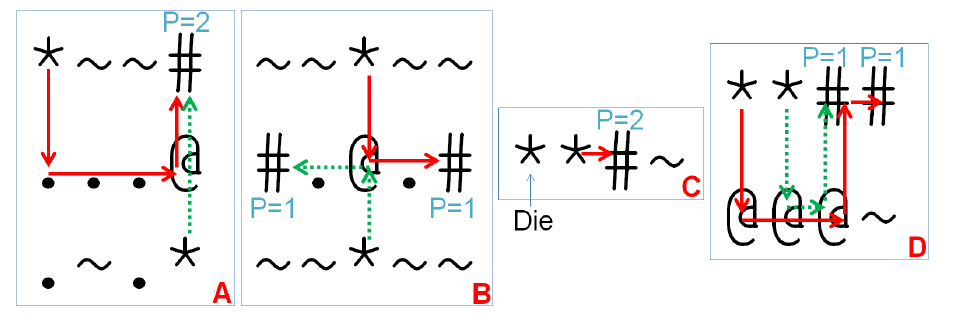
\includegraphics[width=0.7\textwidth]{../img/uva11380_halim}
%   \end{center}
%   \ppagenote{Image from \emph{Competitive Programming, 3rd edition}}
% \end{frame}
%
% \begin{frame}
%   \frametitle{Titanic (UVA11380) -- Network Flow}
%   \begin{block}{Graph Modeling}
%     Number of escaped people = Max Flow of the graph. But how do we create the flow graph?
%   \end{block}
%   One example:
%   \begin{itemize}
%     \item Every non-water cell has two vertices: "In" and "Out";
%     \item Connect "In" and "Out" vertices with cell capacity:
%     \begin{itemize}
%       \item Iceberg and wood: Infinite
%       \item ice and initial position: 1
%     \end{itemize}
%     \item Connect every "Out" vertex with other nearby "In" vertices with infinite capacity;
%     \item Connect "Super Source" with all "initial positions" with capacity 1;
%     \item Connect all "Wood" with "Super Sink", with capacity P.
%   \end{itemize}
% \end{frame}

\begin{frame}
  \frametitle{Prime Pairing -- Bipartite Graph Flow}
  \begin{block}{Problem Description}
    Two numbers $a,b$ are be {\bf prime paired} if $a+b$ is prime.\bigskip

    Given a set of numbers $N$, is it possible to create a {\bf complete pairing} with all elements of $N$?
  \end{block}\bigskip

  Example:
  \begin{itemize}
  \item $N = \{1,4,7,10,11,12\}$
  \item Pairing: $\{1,4\}, \{7,10\}, \{11,12\}$
  \end{itemize}

  \vfill

  Is this even a graph problem??
\end{frame}

\begin{frame}
  \frametitle{Prime Pairing -- Bipartite Graph Flow}
  \begin{block}{Trick}
    It is possible to think of this problem as an {\bf allocation} problem.\bigskip

    Remember that {\bf even + even = even} and {\bf odd + odd = even}. So a prime pair must be one even \# and one odd \#.\bigskip

    In this way, we must allocate even numbers to odd numbers (or vice-versa)
  \end{block}

  How to create the graph:
  \begin{itemize}
  \item Split set between odds and evens;
  \item If \#odd is not equal to \#even, there is no solution;
  \item Create edges between odds and evens if they are a prime pair;
  \item Add a super source and super sink;
  \end{itemize}\bigskip

  If max flow = \# vertices / 2, then there is a solution.
\end{frame}

%\begin{frame}
%  \frametitle{Flow and Special Graph problems}
% %% TODO: Add more special problems from the book for discussion
%\end{frame}
